\chapter{Figures, Tables, and Source Code}
\label{cha:Figures}


Figures and tables are usually placed together with a numbered \emph{caption}
(see Figure~\ref{fig:CocaCola}). The main text \emph{must} contain a
\emph{reference} to each figure and the actual figure should be positioned
\emph{after} the first reference in the \latex source text.

\begin{figure}
    \centering
    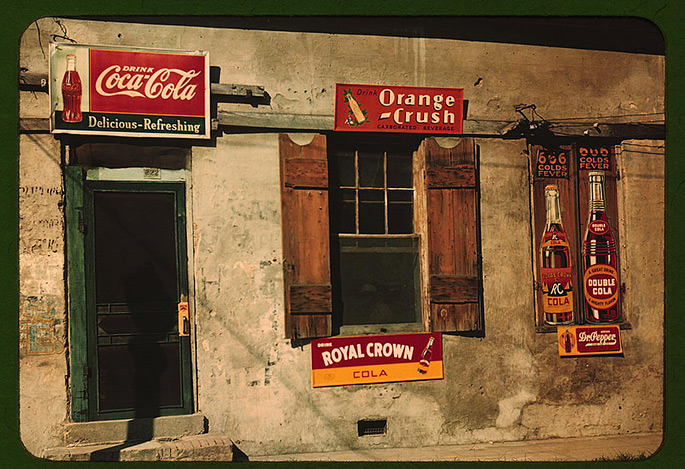
\includegraphics[width=.75\textwidth]{cola-public-domain-photo-p}
    \caption{Coca-Cola Werbung 1940 \cite{CocaCola1940}.}
    \label{fig:CocaCola}
\end{figure}


\section{Let Them Float!}

Placing figures and tables is one of the most difficult tasks in typesetting
because they usually take up a lot of space and often cannot be placed on the
current page in the running text. These elements must therefore be moved to a
suitable place on subsequent pages, which is very tedious to do manually (but
necessary in \emph{Word}, for example).

When positioning these elements, an attempt is made, on the one hand, to
leave as little empty space as possible in the text flow and, on the other
hand, not to move the figures and tables too far away from the original text
passage. In \latex, this works largely automatically by treating figures,
tables and the like as "floating bodies".

The idea that illustrations, for example, will hardly ever fit exactly in the
desired position and possibly not even on the same page may appear strange or
even frightening for many beginners. Nevertheless, for the time being \latex\
should confidently be left to do this work and the author should \emph{not}
manually intervene! Only when the complete document "stands" and the
automatic placement still appears unsatisfactory, interventions in
\emph{individual} situations are justified.%
\footnote{By adding specific placement instructions (see
\cite[p.~39]{Oetiker2021}).}


\section{Captions}

For figures, the caption is usually placed at the \emph{bottom}, while for
tables---depending on the adopted convention---\emph{above} (as in this
document), but sometimes also at the \emph{bottom}. In \latex\ numbering of
figures is also done automatically, as well as the entry into the (optional)
list of figures at the end of the document.%
\footnote{A separate list of figures at the end of the document is easy to
create, but it is unnecessary in a thesis (and everywhere else, actually).
It should therefore be omitted. However, if your advisor insists on it, you can
find instructions on how to add it to your document in the wiki of the
\texttt{hagenberg-thesis} GitHub repository.}

Captions are marked in \latex using the \verb!\label{}! statement, which must
immediately follow the \verb!\caption{}! statement:
%
\begin{LaTeXCode}[numbers=none]
\begin{figure}
    \centering
    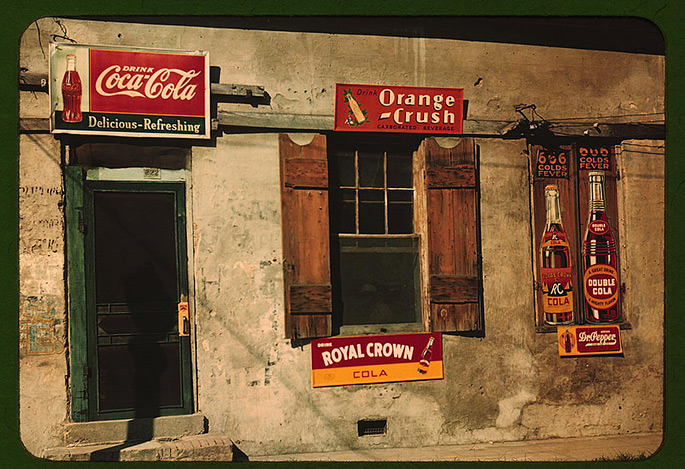
\includegraphics[width=.95\textwidth]{cola-public-domain-photo-p}
    \caption{Coca-Cola Werbung 1940 \cite{CocaCola1940}.}
    \label{fig:CocaCola}
\end{figure}
\end{LaTeXCode}
%
The \emph{name} of the label (\texttt{fig:CocaCola}) can be chosen
arbitrarily. The specific tag "\texttt{fig:}" is (as mentioned in Section
\ref{sec:cross-references}) just a useful aid to better distinguish different
label types when writing.

The length of the captions can be very different. Depending on the
application and style, sometimes a very short caption
(Figure~\ref{fig:CocaCola}) or a longer one (Figure~\ref{fig:ibm360}) results.
Note how short captions are \emph{centered} while long captions use
\emph{justified} formatting (\latex does this automatically). Captions should
\emph{always} end with a period.%
\footnote{Interestingly, some instructions call for the exact opposite,
    supposedly because with classic lead type the final dots are often
    "broken away" in printing. One can believe that or not, but it certainly
    does not matter in digital printing.}

\begin{figure}
    \centering
    \fbox{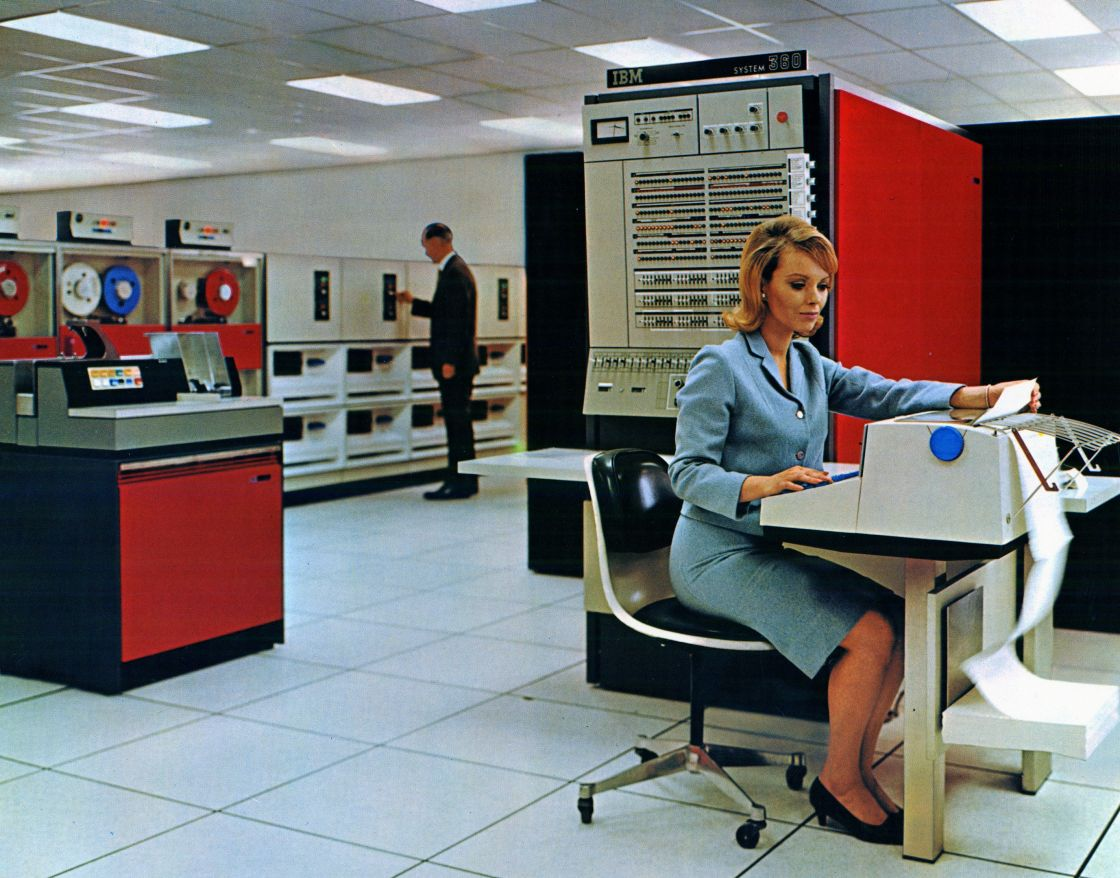
\includegraphics[width=.6\textwidth]{ibm-360-color}}
    \caption{Example of a long caption text. \textsc{Univac} launched the
    Model 751, the first high-performance computer with semiconductor memory,
        in 1961. More than fifty of these computers were sold in the U.S.A.\
        in the first year of production, primarily to military agencies,
        insurance companies, and major banks. It was replaced two years later
        by the Model 820, developed in cooperation with \textsc{Sperry}. This
        may sound plausible, but it is complete nonsense, and the picture
        actually shows a System/360 mainframe computer from IBM. Image
        source~\cite{IBM360}.}
    \label{fig:ibm360}
\end{figure}


\section{Figures}

For the inclusion of graphics in \latex the use of the
standard package \texttt{graphicx} \cite{Carlisle2024} is recommended
(automatically loaded by the \texttt{hagenberg-thesis} package).
With the current workflow (using \texttt{pdflatex}) images and graphics
can only be included in the following formats:
%
\begin{itemize}
    \item PNG: for gray, B/W and color raster images (preferred),
    \item JPEG: for photographs (if not otherwise available),
    \item PDF: for vector graphics (illustrations, line drawings \etc).
\end{itemize}
%
For raster images, PNG should be used if possible, because the images it
contains are compressed losslessly and therefore do not have any visible
compression artifacts. In contrast, JPEG should only be used if the original
material (photo) is already available in this format.


\subsection{Where Are Graphic Files Located?}

Images and graphics are usually stored in a subdirectory (or several
subdirectories), in the case of this document in \nolinkurl{images/}. This is
done by the following statement at the beginning of the main document
\nolinkurl{main.tex} (see also Appendix \ref{app:latex}):
%
\begin{GenericCode}[numbers=none]
\graphicspath{{images/}}
\end{GenericCode}
%
The path \texttt{graphicspath} (relative to the main document) can be changed
at any time within the document, which is quite useful if, \eg, the graphics
of individual chapters are to be stored separately in corresponding directories.


\subsection{Adjusting Picture Size}

The \emph{size} of the printed picture can be controlled by specifying a
certain width or height or a scaling factor, \eg:
%
\begin{GenericCode}[numbers=none]
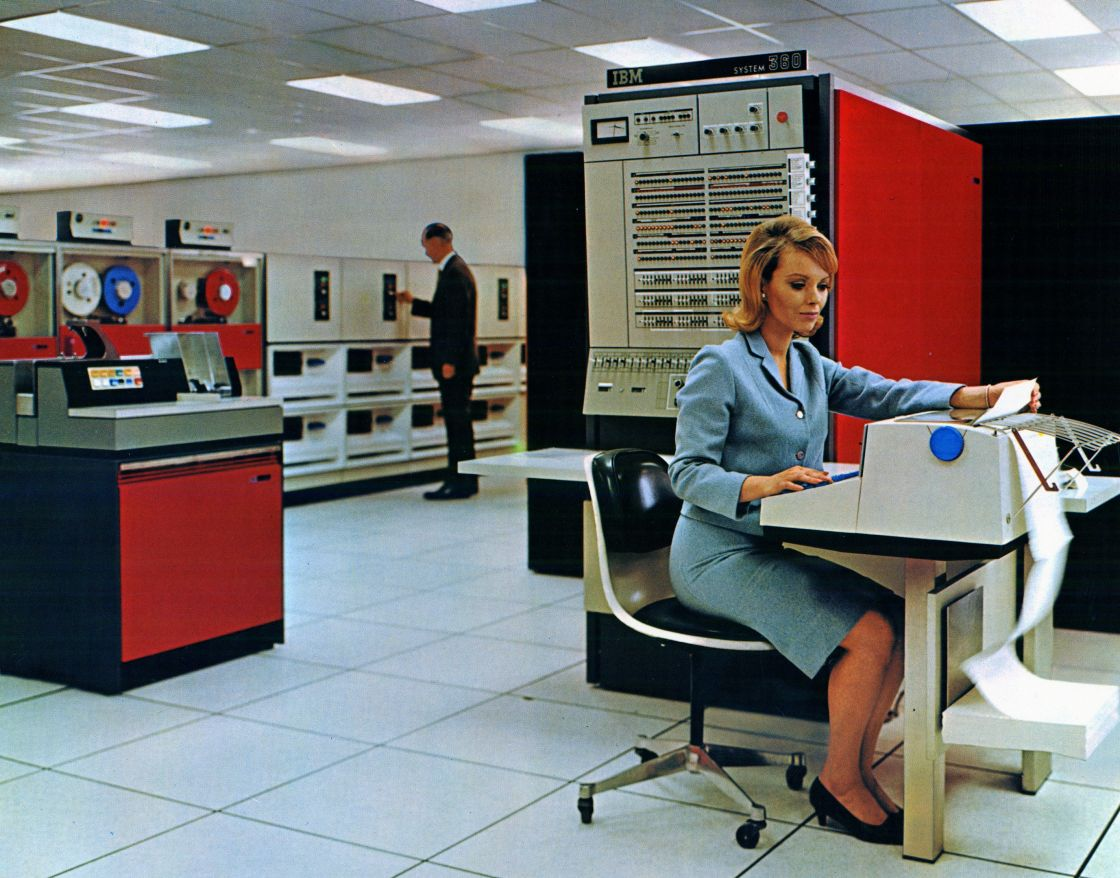
\includegraphics[width=.85\textwidth]{ibm-360-color}
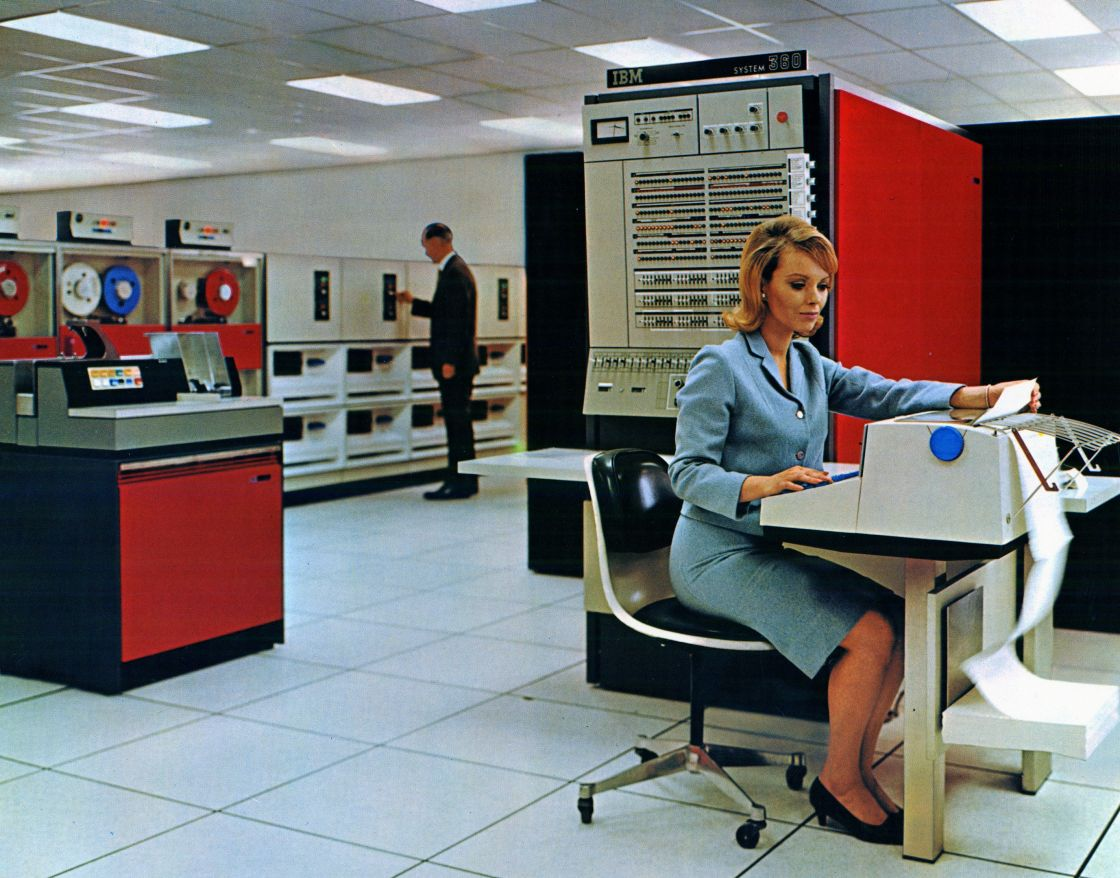
\includegraphics[scale=1.5]{ibm-360-color}
\end{GenericCode}
%
Note that file extensions need not be explicitly specified.
This is particularly convenient when multiple workflows with different file
types are used.


\subsection{Framing Graphics}

The macro \verb!\fbox{...}! can optionally be used to create a thin frame
around the graphic, for example:
%
\begin{GenericCode}[numbers=none]
\fbox{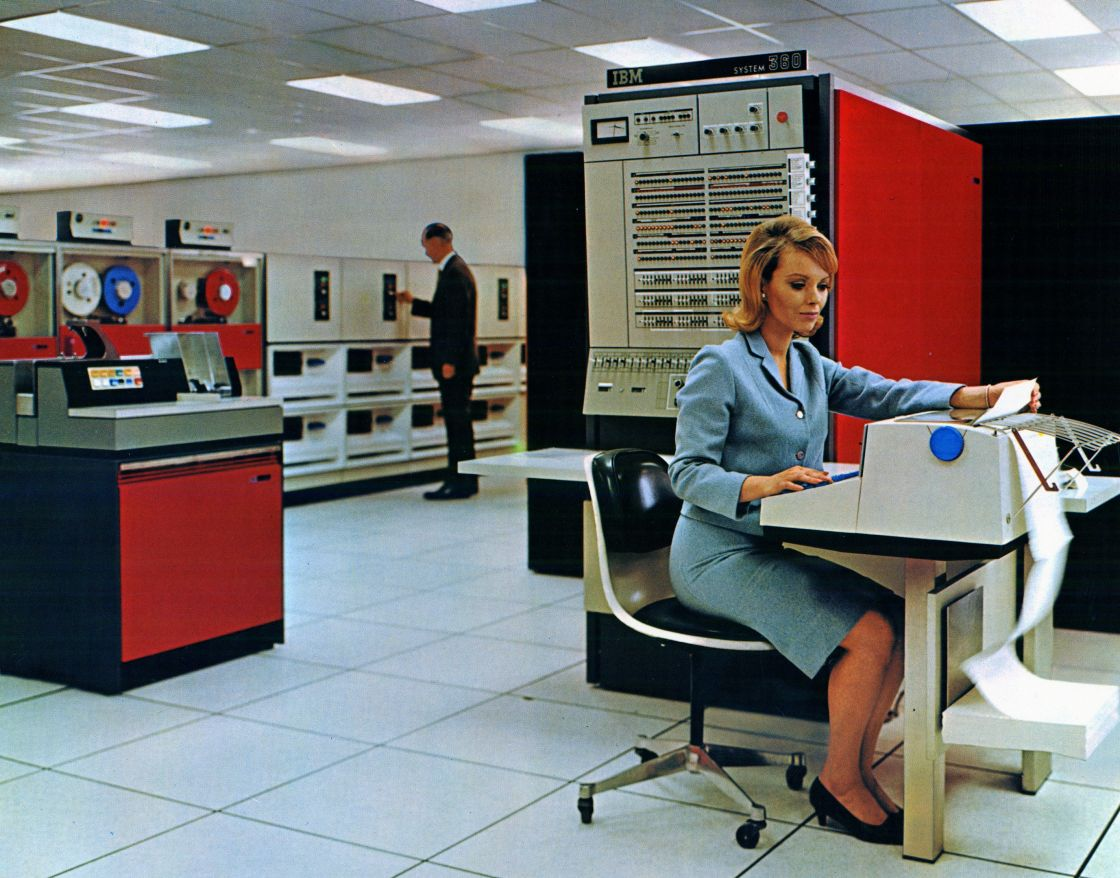
\includegraphics[height=50mm]{ibm-360-color}}
\end{GenericCode}
%
This is usually only necessary for raster images, especially if they are very
bright towards the edge and would not be distinguishable from the background
without a frame.

\subsection{Raster (Pixel) Praphics}

In general, raster images should be prepared in advance so that they lose as
little quality as possible when printed later. It is therefore advisable to
set the image size (resolution) correctly in advance (\eg\ with
\emph{Photoshop}). Common resolutions related to the final image size are:
%
\begin{itemize}
    \item color and gray scale images: 150--300 dpi,
    \item binary (black/white) images: 300--600 dpi.
\end{itemize}
%
A much higher resolution does not make sense due to the screening required in
laser printing, even with 1200 dpi printers. Especially \emph{screen\-shots}
should not be displayed too small, otherwise they are hard to read (max.\ 200
dpi, better 150 dpi). Consider that the work should still be legible in all
details even as a photocopy.

\subsubsection{Careful With JPEG!}

As a rule, images intended for use in print documents should never be saved
using lossy compression methods. In particular, the use of JPEG should be
avoided if possible, even if it makes many files much smaller. The exception
is when the original data is only available in JPEG and has not been edited
or resized for embedding. Otherwise, PNG should always be used.

Often color screenshots are subjected to JPEG compression, although its
devastating consequences should be visible to anyone (see
Figure~\ref{fig:jpeg-bungle}).%
\footnote{The JPEG process is designed for \emph{natural} photos and should
only be used for these.}

\begin{figure}
    \centering\small
    \begin{tabular}{@{}cc@{}}
        \fbox{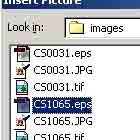
\includegraphics[width=0.475\textwidth]{screenshot-dirty}} &
        % JPEG file
        \fbox{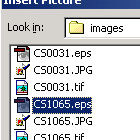
\includegraphics[width=0.475\textwidth]{screenshot-clean}} \\
        % PNG file
        (a) JPEG & (b) PNG
    \end{tabular}
    \caption{Typical JPEG bungle.
    Screenshots and similar raster images available as originals should
    \emph{never} be compressed with JPEG for print documents.
    The result~(a) not only looks dirty compared to the uncompressed
    original~(b), but may also become illegible in print.}
    \label{fig:jpeg-bungle}
\end{figure}

\subsection{Vector (Line) Graphics}

For illustrations and schematic diagrams (\zB flowcharts, entity-relationship
diagrams or other structural representations), vector graphics (PDF) should
always be used. Rasterized graphics, as they are usually available as GIF or
PNG files on web pages, have no place in a print document; if necessary they
must be re-drawn with an appropriate vector graphics tool (of course not
without referencing the original source).

In this case, PDF is really the only choice, being a universal and
standardized container format for many other applications. A suitable
graphics program, \eg, \emph{Adobe Illustrator} or \emph{Inkscape}, is
required to create PDF vector graphics. Note that some popular tools do not
support direct export of PDF files or generate unclean files. Before deciding
on a particular drawing software, this should be tried out in case of doubt.
If everything else fails, PDFs can also be generated by most printer drivers.

\subsubsection{Font Embedding in Graphics}

The rendering of text elements depends on the fonts installed on the computer
(or printer) and the form of font embedding in the source document. Correct
display on the screen of your computer does not mean that the same document
will be displayed exactly the same way on another computer or printer. This
consideration is particularly important when print documents are made
available online. Therefore, make sure that the fonts used in your graphics
appear exactly as intended in the printout (see also Section
\ref{sec:TexFontsInGraphics}).

\subsubsection{Stroke Widths -- Avoid \emph{Hairlines}!}

In graphics programs such as \emph{Illustrator} and \emph{Inkscape}, which
are essentially based on PDF or SVG functionality, it is possible to define
lines in terms of their thickness as "hairlines". This should produce "as
thin as possible" lines in the output. The result depends exclusively on the
respective printer and is therefore hardly predictable. \emph{Conclusion:}
Avoid hairlines and always use concrete line widths ($\geq 0.25\,
\mathrm{pt}$) instead!

\subsection{Using \tex\ Fonts in Graphics}
\label{sec:TexFontsInGraphics}

As a general rule, fonts used in graphics should match the typography of the
main text as closely as possible. An interesting tool for this is \emph{Ipe
Extensible Drawing Editor},%
\footnote{\url{https://ipe.otfried.org/}}
a drawing program that generates text in graphics directly with \latex\
(including mathematical expressions) and uses PDF as its native file format.
For images created with other external graphics programs, you can use at
least \emph{similarly} looking fonts (like \emph{Times-Roman} or
\emph{Garamond}). However, it is also possible to use the
\emph{Computer-Modern} (CM) font family from {\tex}/{\latex} directly to
generate graphics. Some ports of CM are available as \emph{TrueType} fonts,
which can also be used in conventional graphics programs under \emph{Windows}
and \emph{macOS}:
%
\begin{itemize}
    \item
    Recommendable is the "BaKoMa Fonts Collection",%
    \footnote{\url{http://ctan.org/pkg/bakoma-fonts}}
    which contains (beside the CM standard fonts) also the mathematical fonts
    of the
    AMS family.
    \item
    Another option are the "LM-Roman" Open-Type fonts,%
    \footnote{\url{http://www.gust.org.pl/projects/e-foundry/latin-modern}}
    which were specifically developed for use in the \latex environment.
    They are also part of the standard \latex distributions, such as MikTeX.
    These fonts include dedicated glyphs for "umlauts" and are therefore well
    suited for German texts as well.
\end{itemize}
%
Of course, these fonts must first be installed on your computer before 
you can use them.

\subsection{Grapics With \latex Overlays (Using \texttt{overpic})}
\label{sec:GraphicOverlays}

Sometimes it is necessary to overlay an existing image or graphic with
\latex's own (vector) elements, \eg, for markers or labels. A typical example
is shown in Figure~\ref{fig:overpic-example} where a PDF graphic created with
\emph{Mathematica} is annotated with mathematical text elements. This is
accomplished using the \texttt{overpic} package, where the underlying graphic
is not imported with \verb!\includegraphics! but \verb!\begin{overpic}!
\ldots \verb!\end{overpic}!, with a similar syntax:
%
\begin{LaTeXCode}[numbers=none]
\begin{overpic}[width=0.85\textwidth]{mathematica-example}
    \put(101,14){$x$}%
    \put(4,31){$f(x)$}%
    \put(29.5,28){\line(1,1){2}}%
    ...
\end{overpic}
\end{LaTeXCode}

\begin{figure}
    \centering\small
    \vspace*{3mm}
    \begin{overpic}[width=0.85\textwidth]{mathematica-example}
        \put(101,14){$x$}%
        \put(4,31){$f(x)$}%
        \put(29.5,28){\line(1,1){2}}%
        {\color{green!70!black}\put(29.5,28){\circle*{2.0}}}%
        \put(32,30){$\cos(\frac{7}{3} x)$}%
        \put(59,28){\line(1,1){2}}%
        {\color{blue!70!black}\put(59,28){\circle*{2.0}}}%
        \put(61.5,30){$\cos(x)$}%
    \end{overpic}
    \caption{Example of using the \texttt{overpic} package to insert \latex
    elements over an imported graphic. In this case, the mathematical
    elements $x$, $f(x)$, $\cos(x)$ and $\smash{\cos(\frac{7}{3} x)}$ as well
    as two diagonal straight lines and filled (colored) circles were inserted
    . All this is drawn on top of a vector graphic imported from file
    \texttt{mathematica-example.pdf}.}
    \label{fig:overpic-example}
\end{figure}

The \texttt{overpic} environment also forms a \texttt{picture} environment%
\footnote{\url{https://www.overleaf.com/learn/latex/Picture_environment}}
where \latex drawing instructions (such as \verb!\put! and the like) can be
placed, as shown in Figure~\ref{fig:overpic-example}.%
\footnote{The default drawing instructions in \latex are quite restrictive,
so the \texttt{pict2e} package is additionally used (see
\url{https://ctan.org/pkg/pict2e}).}
The $x/y$ positions are specified as a percentage of the image width. Further
details can be found in the source code.

\subsection{Figures With Multiple Elements}

If multiple images or graphics are combined into one figure, a common caption
is typically used, as shown in Figure~\ref{fig:Bearings}. In the main text, a
reference to a particular part of the figure, such as the single-row roller
bearing in Figure~\ref{fig:Bearings}\,(c), could look like this:
%
\begin{LaTeXCode}[numbers=none]
... Figure~\ref{fig:Bearings} (c) ...
\end{LaTeXCode}

\subsection{Source Citations in Captions}
\label{sec:SourceCitationsInCaptions}

If images, graphics or tables from other sources are used, then their origin
must be made clear in any case, and preferably directly in the caption. For
example, if an illustration from a book or other citable publication is used,
then it should be included in the bibliography and cited as usual with
\verb!\cite{..}! as demonstrated in Fig.\ \ref{fig:Bearings}. Further details
on this type of source citation can be found in Chapter~\ref{cha:Literature}
(esp.\ Section~\ref{sec:category-online}).

\begin{figure}
    \centering\small
    \begin{tabular}{@{}c@{\hspace{12mm}}c@{}} % mittlerer Abstand = 12mm
        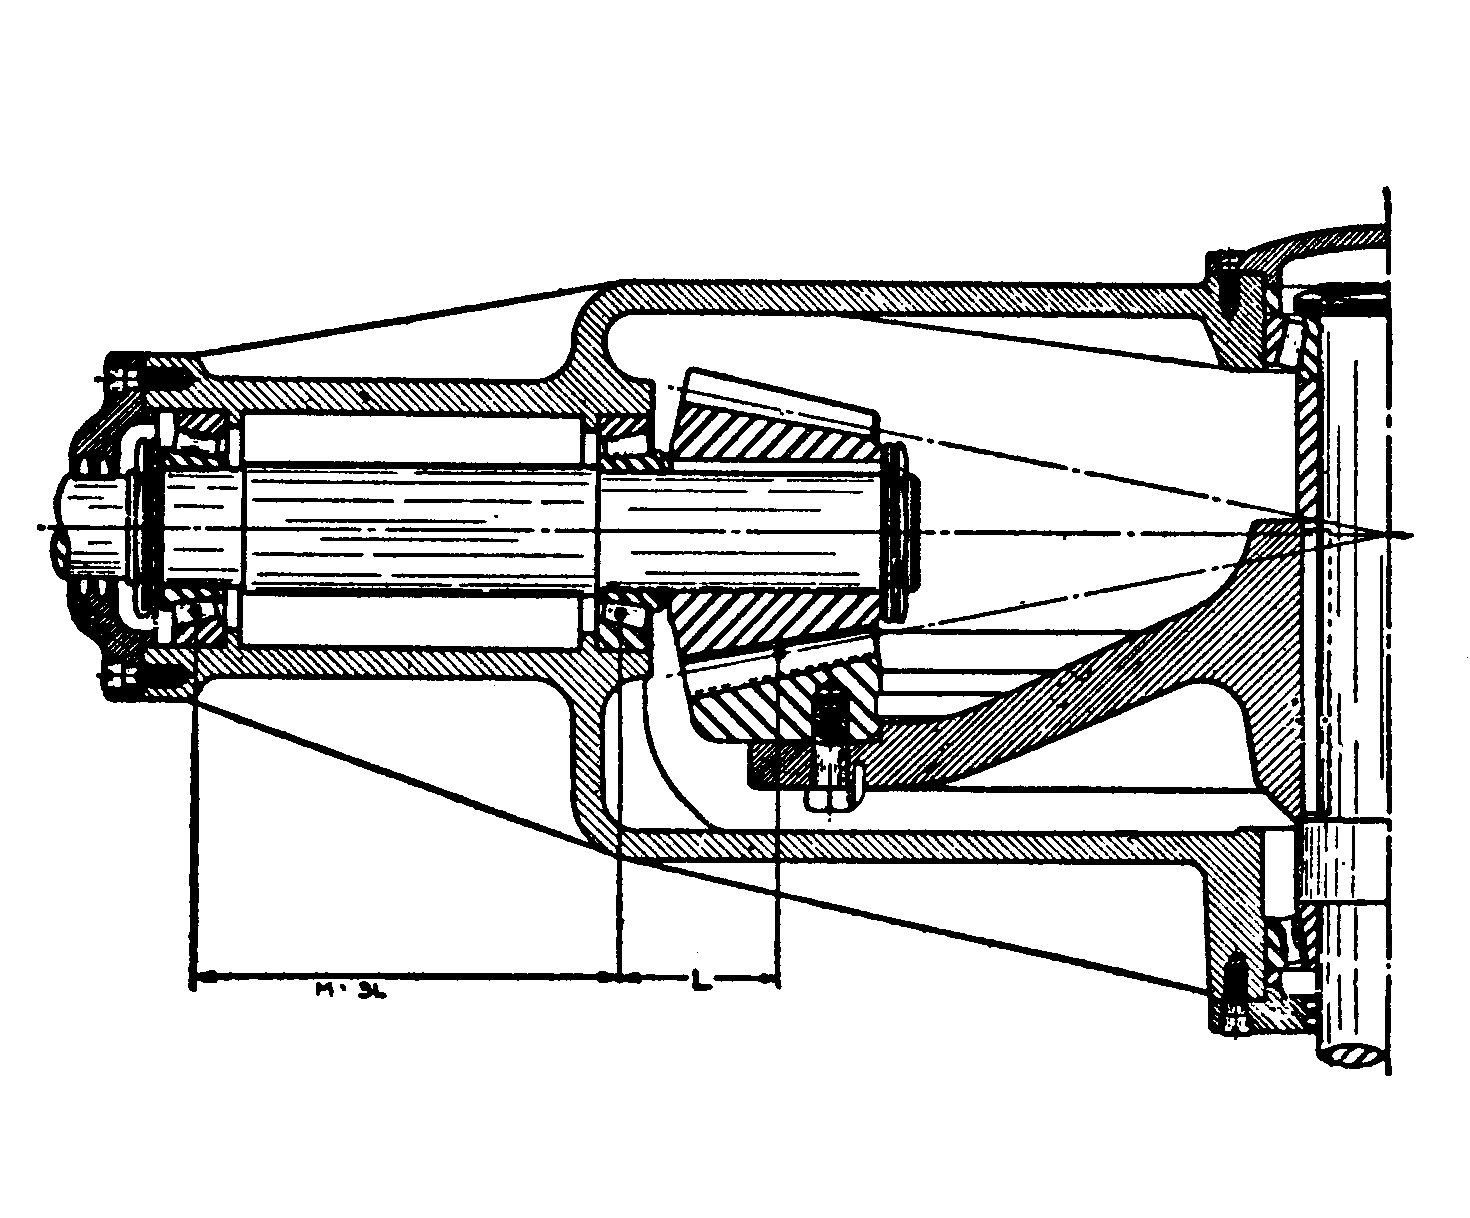
\includegraphics[width=.45\textwidth]{overhang-mounting} &
        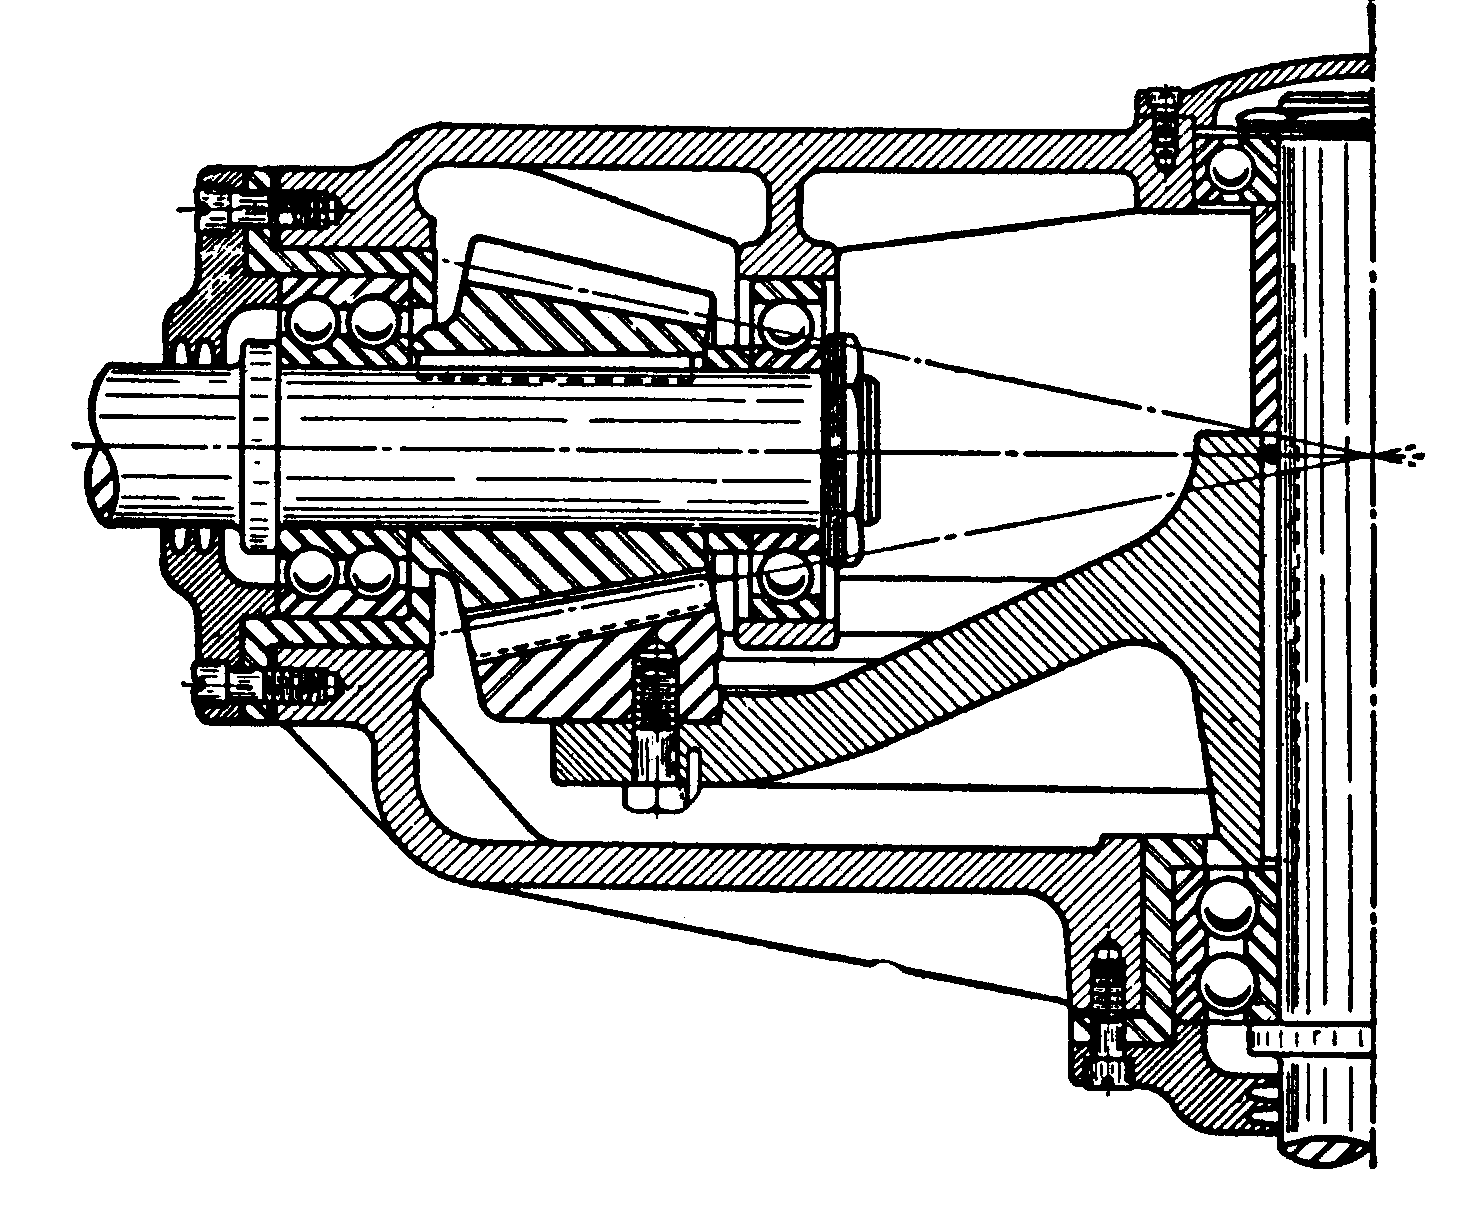
\includegraphics[width=.45\textwidth]{straddle-mounting}
        \\
        (a) & (b)
        \\[4pt]    %vertical extra spacing (4 points)
        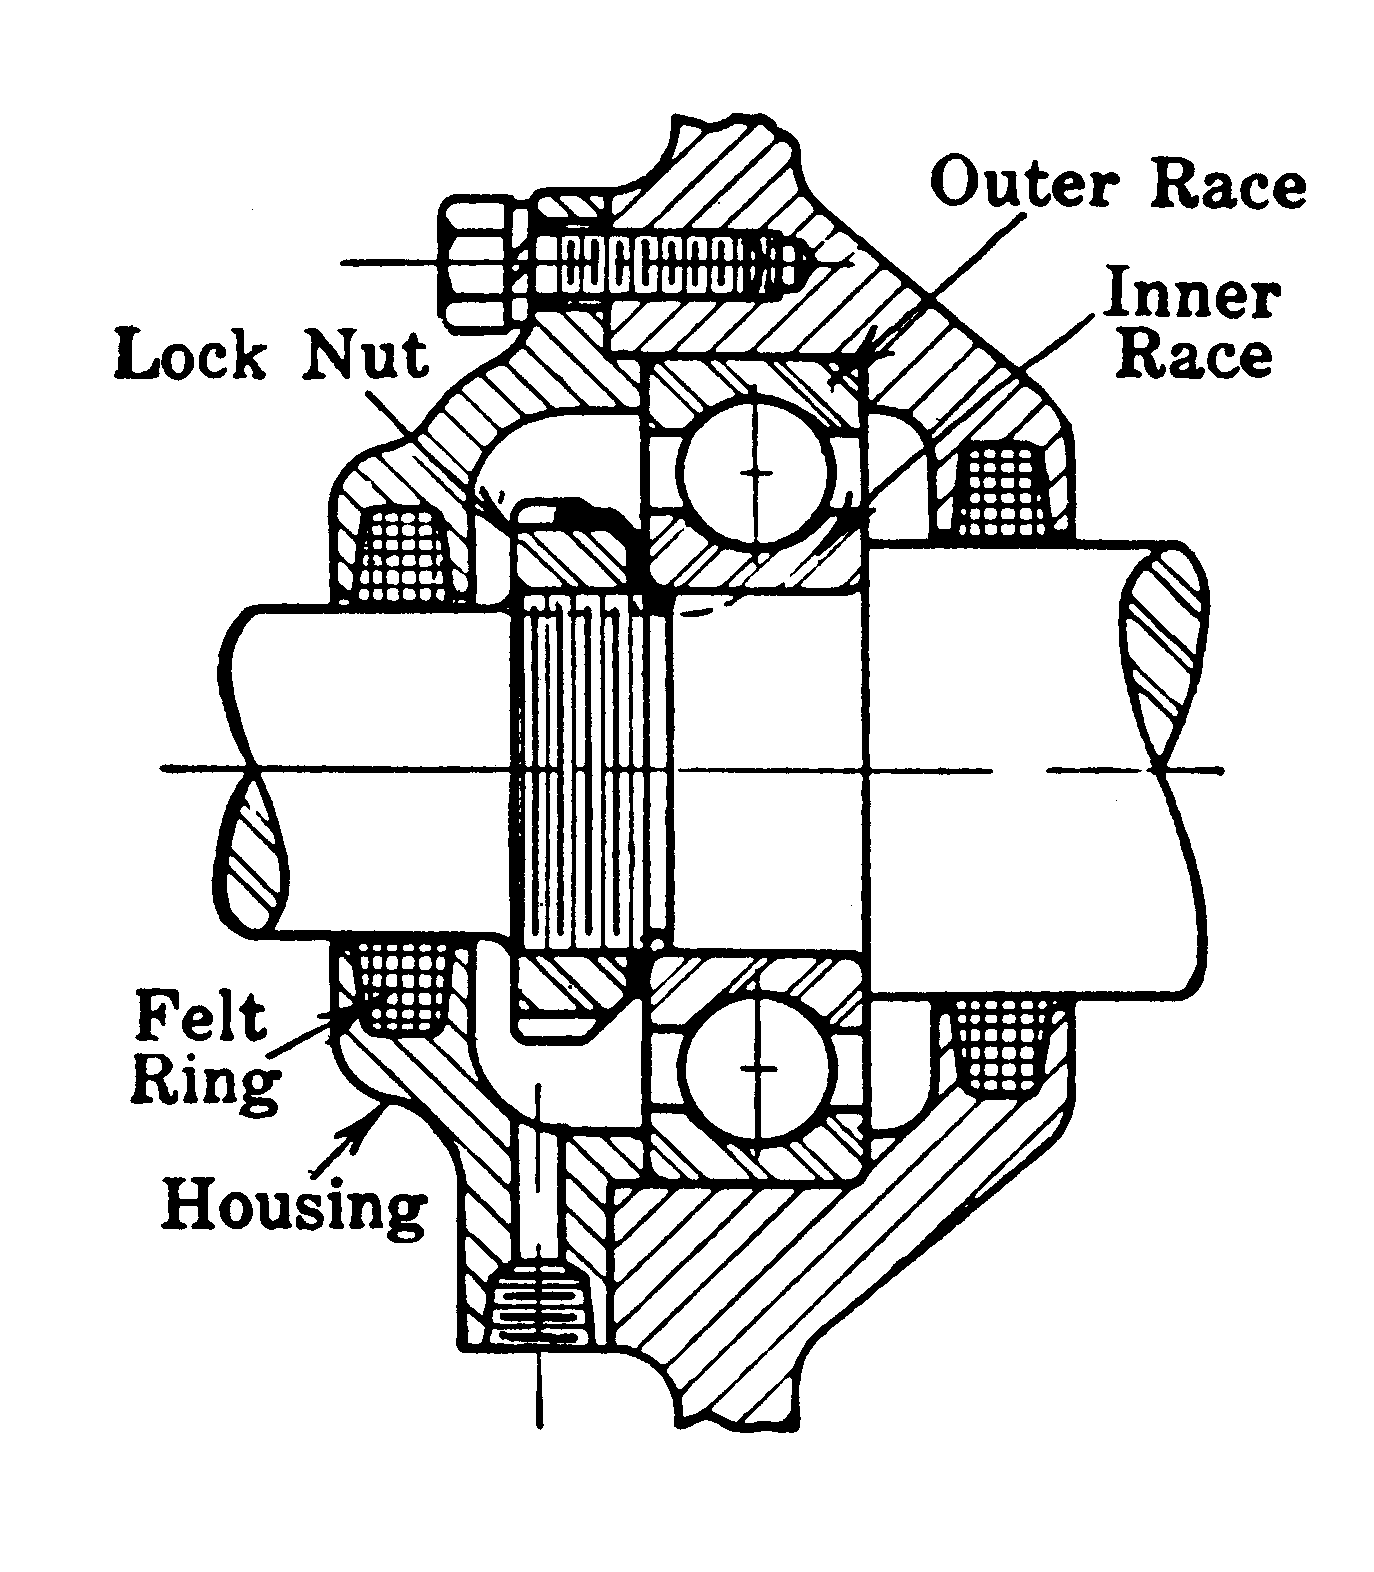
\includegraphics[width=.45\textwidth]{ball-bearing-1} &
        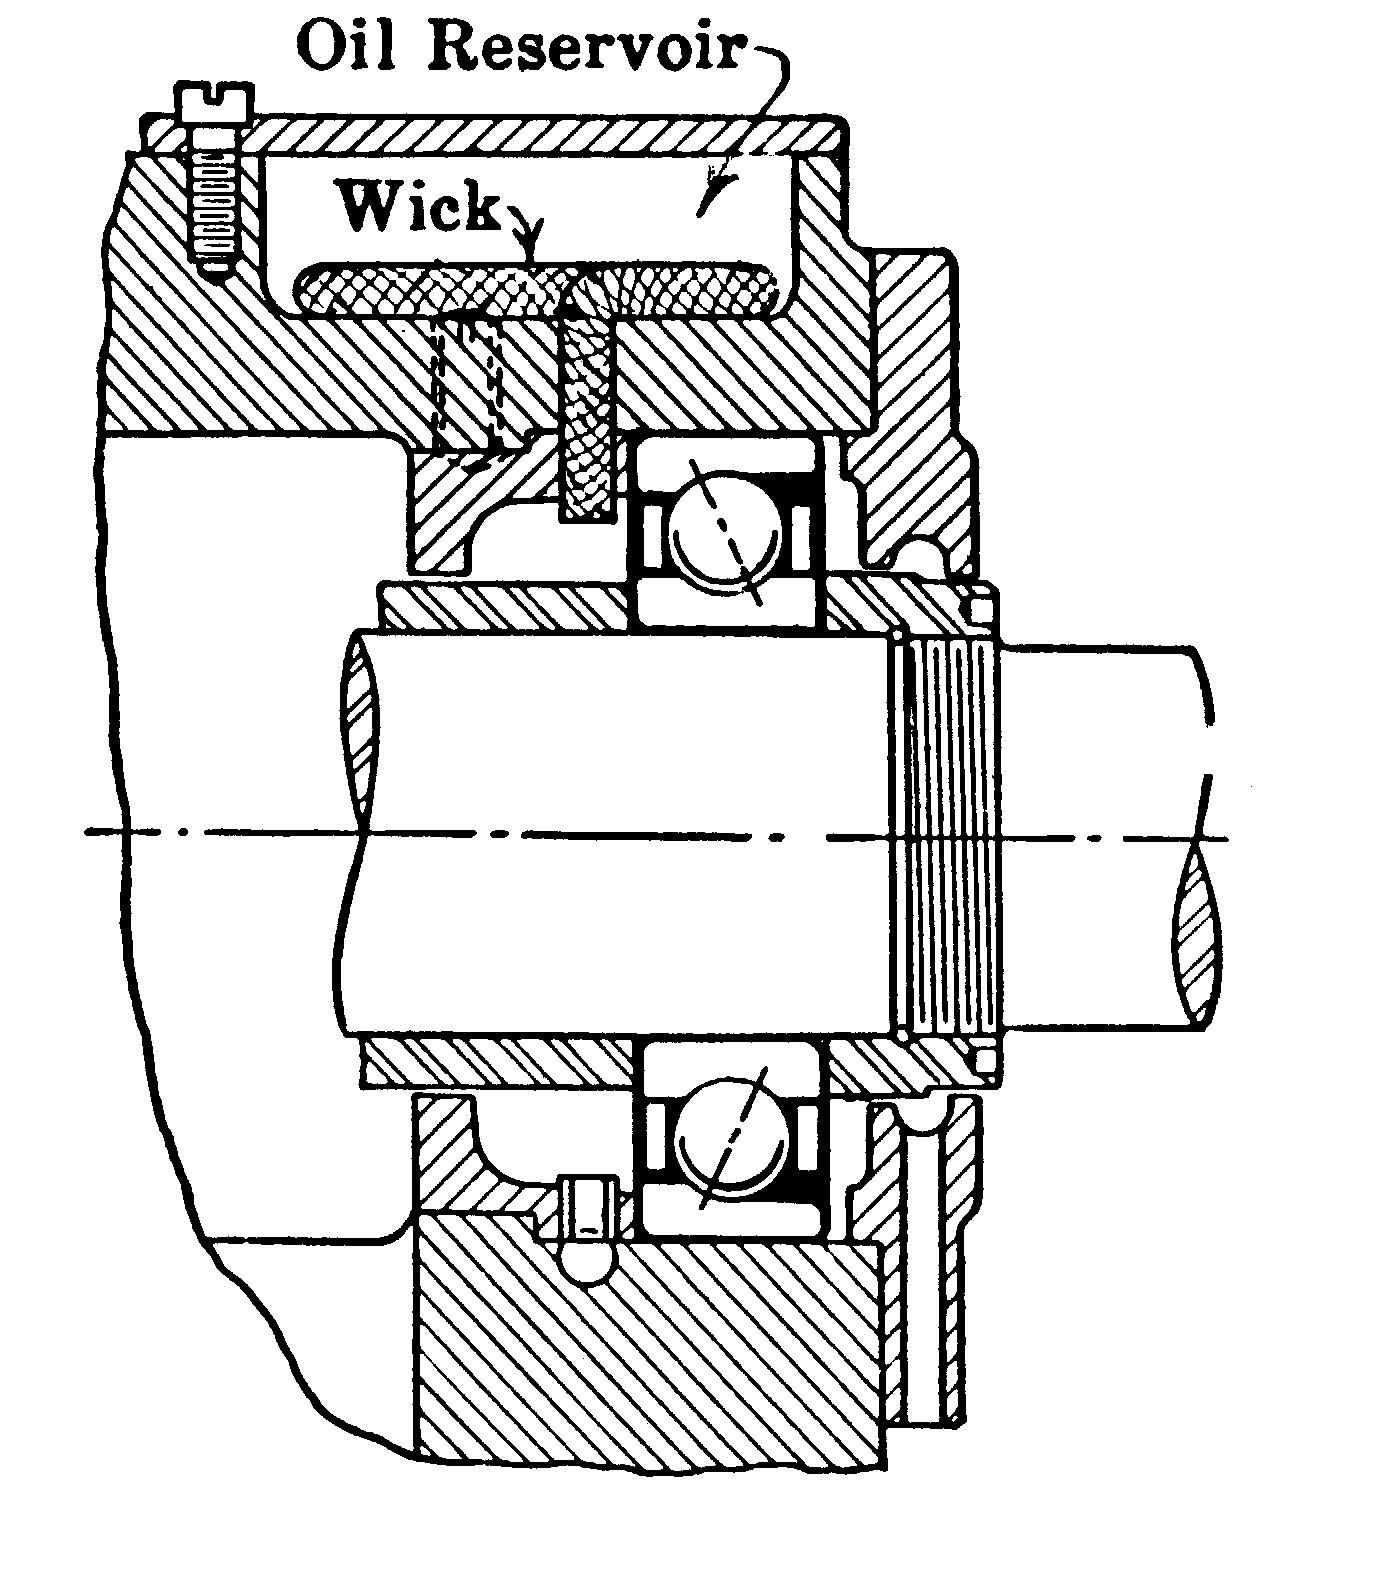
\includegraphics[width=.45\textwidth]{ball-bearing-2}
        \\
        (c) & (d)
    \end{tabular}
%
\caption{Various machine elements in an illustration with multiple elements.
\emph{Overhang mounting}~(a), \emph{straddle mounting}~(b), single row roller
bearing~(c), lubrication of roller bearings~(d). This figure uses an ordinary
table (\texttt{tabular}) with 2 columns and 4 rows (details can be found in
the source code). Image source~\cite{Faires1934}.}
\label{fig:Bearings}
\end{figure}

In the case of images created using AI tools, however, a classic reference in
the bibliography makes little sense. Instead, the tool used and the prompt
entered should be stated in the caption, as shown in Figure
\ref{fig:ai-tool-image}.

\begin{figure}
	\centering
	
\includegraphics[width=.5\textwidth]{ai-tool-image}
	\caption{Example of an image created using an AI tool. Source:
    DALL$\cdot$E 3 using the prompt "Create a    photorealistic image of the
    following scenario: a female student sits in front of her desktop computer
    and writes her thesis in LaTeX".}
	\label{fig:ai-tool-image}
\end{figure}


\section{Tables}
\label{sec:Tables}

Tables are often used to present numerical relationships, test results, etc.\
in a clear form. A simple example is Table~\ref{tab:programming-languages},
the associated \latex source can be found in 
Program~\ref{prog:programming-languages-source}.

As arguments of the \texttt{tabular} environment the alignments of the
individual columns are specified. The number of arguments thus determines the
number of columns. Valid items are \texttt{l} for left-aligned, \texttt{c}
for centered, and \texttt{r} for right-aligned. The column width results from
the length of the contents, there are no automatic line breaks. To set the
width and thus create automatic line wraps, \verb|p{width}| (paragraph mode)
is used, where \texttt{width} is a valid length specification (see
\cite{WikibooksLaTeXLengths2018} for details). The \verb|@{}| items remove
the (usually unwanted) margin at the left and right table borders.

\begin{table}
    \caption{Programming languages at a glance.}
    \label{tab:programming-languages}
    \centering
    \setlength{\tabcolsep}{10pt} 				% separator between columns (standard = 6pt)
    \renewcommand{\arraystretch}{1.25}	% vertical stretch factor (standard = 1.0)
    \begin{tabular}{@{}llll@{}}
        \toprule
        Language   & Type        & Typical Use      & Standards          \\
        \midrule
        C++        & Compiled    & Applications     & ISO/IEC 14882:2020 \\
        COBOL      & Compiled    & Business         & ISO/IEC 1989:2014  \\
        JavaScript & Interpreted & Web              & ECMA-262           \\
        Python     & Interpreted & Machine Learning & PEPs               \\
        \bottomrule
    \end{tabular}
\end{table}

\begin{program}
% place caption consistently either at the top or bottom:
    \caption{\latex\ source code for Table \ref{tab:programming-languages}.
    The generation of the displayed listing itself is described in
    Section~\ref{sec:program-texts}.}
    \label{prog:programming-languages-source}
%
\begin{LaTeXCode}[numbers=none]
\begin{table}
    \caption{Programming languages at a glance.}
    \label{tab:programming-languages}
    \centering
    \setlength{\tabcolsep}{10pt} % separator between columns (standard = 6pt)
    \renewcommand{\arraystretch}{1.25} % vertical stretch factor (standard = 1.0)
    \begin{tabular}{@{}llll@{}}
        \toprule
        Language   & Type        & Typical Use      & Standards          \\
        \midrule
        C++        & Compiled    & Applications     & ISO/IEC 14882:2020 \\
        COBOL      & Compiled    & Business         & ISO/IEC 1989:2014  \\
        JavaScript & Interpreted & Web              & ECMA-262           \\
        Python     & Interpreted & Machine Learning & PEPs               \\
        \bottomrule
    \end{tabular}
\end{table}
\end{LaTeXCode}
%
\end{program}

The demand for an attractive appearance of tables has increased noticeably in
recent years. For example, many authors and publishers using \latex now
follow some simple design guidelines for tables \cite{Fear2020}, of which
particularly the first two determine their basic layout:

\begin{enumerate}
    \item Never use vertical lines.
    \item Never use double lines.
    \item Place units in the column header (not in the table content area).
    \item A decimal separator is always preceded by a digit; thus write
    "$0{,}1$" not just "${,}1$".
\end{enumerate}


The \latex package \texttt{booktabs} makes it easy to meet these requirements
Within the \texttt{tabular} environment (which defines the actual table), the
number of columns---preferably set left-justified (\texttt{l}
specifiers)--- are defined first. \verb|\toprule| marks the beginning of the
table, followed by the header, which is terminated by \verb|\midrule|. This is
followed by the lines with the table contents. Using \verb|\bottomrule| the
table is closed with another horizontal line. \verb|\midrule| calls can also
occur more often to divide the table. If horizontal lines are needed that should
not span all columns, \verb|\cmidrule| can be used.

\subsection{Long Texts in Table Columns}

Sometimes it is necessary to fit relatively large amounts of text into narrow
columns in tables, as in Table \ref{tab:synthesis-techniques}. In this case,
it makes sense to go without justification and at the same time relax the
strict hyphenation rules. Details can be found in the corresponding \latex
source text.


%--------------------------------------------------------------------------------
% Table with narrow columns
%--------------------------------------------------------------------------------
\begin{table}
    \caption{Example of a table with multiline text in narrow columns.
    Here the columns are too narrow for justification, so left alignment
        ("ragged-right") is used.}
    \label{tab:synthesis-techniques}
    \centering
    \newcommand{\RR}{\rightskip=0pt plus1em \spaceskip=.3333em \xspaceskip=.5em\relax}
    \renewcommand{\arraystretch}{1.20}
    \small
    \begin{english}
        \begin{tabular}{@{}p{0.2\textwidth}lp{0.3\textwidth}p{0.2\textwidth}@{}}
            \toprule
            Method & Implem. & Features & Status \\
            \midrule
            {\RR polygon shading} &
            SW/HW &
                {\RR flat-shaded polygons} &
            \\
            {\RR flat shading with z-buffer} &
            SW/HW &
                {\RR depth values} &
            \\
            {\RR goraud shading with z-buffer} &
            SW/HW &
                {\RR smooth shading, simple fog, point light sources} &
                {\RR SGI entry models} \\
            {\RR phong shading with z-buffer} &
            SW/HW &
                {\RR highlights} &
            \\
            {\RR texture mapping with z-buffer} &
            SW/HW &
                {\RR surface textures, simple shadows} &
                {\RR SGI high end, flight simulators} \\
            \bottomrule
        \end{tabular}
    \end{english}
\end{table}


\subsection{Multipage Tables}

Often tabular information needs more than one page. Here the float-element
created by the \texttt{table} environment becomes a problem, because it
prevents breaks across multiple pages. To allow page breaks \emph{within}
tables, the \texttt{longtable} package can be used.%
\footnote{%
\url{http://mirrors.ctan.org/macros/latex/required/tools/longtable.pdf}}
It replaces the \texttt{tabular} environment and does not require a
surrounding \texttt{table} environment.%
\footnote{Note that a \texttt{longtable} is \emph{no} float element but 
always gets inserted at the current text position. This may lead to large
empty blocks if the table header and/or the first table row do not fit onto
the current page.}

The table definition is largely the same as shown in Program
\ref{prog:programming-languages-source}. Only the commands \verb|\endhead|
and \verb|\endfoot| are added. They outline the head and footer areas to be
repeated on each page. If these should be different for the header on the
first page and the footer on the last page, \verb|\endfirsthead| and
\verb|\endlastfoot| are used.

Table \ref{tab:LongtableDemo} shows a concrete example for using 
\texttt{longtable}. A specific header is assigned to the first page, 
defining the main caption text and the associated label.
The following pages show an abbreviated header ("\emph{continued}") with the
\emph{same} table number, which is only defined once in the main header. 
If horizontal and vertical spacing are to be modified, these statements must
be placed \emph{before} the beginning of the table and enclosed with
\verb|{|\ldots\verb|}| or \verb|\begin{block}| \ldots \verb|\end{block}|%
\footnote{The (dummy) "\texttt{block}" environment is defined in 
\texttt{hgb.sty}. It does nothing but provides a limited scope for
temporarily setting (and automatically resetting) \latex\ variables.}
to restrict their scope. Consult the source code of this document for
additional details.

\begin{block}										 % 'block' environment is defined in hgb.sty
\setlength{\tabcolsep}{10pt}     % separator between columns (standard = 6pt)
\renewcommand{\arraystretch}{1.50} % vertical stretch factor (standard = 1.0)
\begin{longtable}{@{}lp{0.23\textwidth}@{}}
		% -------------------------- first header ----------------------------
    \caption{A long table (using \texttt{longtable}) that breaks over two pages. 
		Note that different table headers are defined for the first page and
		subsequent pages and the associated label is only assigned once 
		(referring to \emph{this} page).} 
		\label{tab:LongtableDemo}																						 \\
    \toprule
    First Column            & Second Column                              \\
    \midrule
		\endfirsthead
		% ---------------------- subsequent headers ---------------------------
		\caption*{\textbf{Table \getcurrentlabel} (\emph{continued})}				 \\
    \toprule
    First Column            & Second Column                              \\
    \midrule
		\endhead
		% --------------------------------------------------------------------
    The column on the right contains a lot of text. &
    There is a lot of text in this column, which creates a long column.
    Here, too, it can make sense to set the content left-aligned. However,
    \texttt{longtable} does not wrap lines in such columns, only between
    individual lines. \\
    More lines follow here. & This content serves only as a placeholder. \\
    More lines follow here. & This content serves only as a placeholder. \\
    More lines follow here. & This content serves only as a placeholder. \\
    More lines follow here. & This content serves only as a placeholder. \\
    More lines follow here. & This content serves only as a placeholder. \\
    More lines follow here. & This content serves only as a placeholder. \\
    More lines follow here. & This content serves only as a placeholder. \\
    More lines follow here. & This content serves only as a placeholder. \\
    More lines follow here. & This content serves only as a placeholder. \\
		More lines follow here. & This content serves only as a placeholder. \\
    More lines follow here. & This content serves only as a placeholder. \\
    More lines follow here. & This content serves only as a placeholder. \\
    More lines follow here. & This content serves only as a placeholder. \\
    More lines follow here. & This content serves only as a placeholder. \\
    More lines follow here. & This content serves only as a placeholder. \\
    More lines follow here. & This content serves only as a placeholder. \\
    More lines follow here. & This content serves only as a placeholder. \\
    More lines follow here. & This content serves only as a placeholder. \\
    \bottomrule
\end{longtable}
\end{block}

%{\setlength{\tabcolsep}{10pt} % separator between columns (standard = 6pt)
%\def\arraystretch{1.50}      % vertical stretch factor (standard = 1.0)
%\begin{longtable}{@{}lp{0.23\textwidth}@{}}
    %\caption{A long table that potentially breaks over two pages.} \\
    %\toprule
    %First Column            & Second Column                              \\
    %\midrule\endhead
    %\label{tab:LongtableDemo}
    %The column on the right contains a lot of text. &
    %There is a lot of text in this column, which creates a long column.
    %Here, too, it can make sense to set the content left-aligned. However,
    %\texttt{longtable} does not wrap lines in such columns, only between
    %individual lines. \\
    %More lines follow here. & This content serves only as a placeholder. \\
    %More lines follow here. & This content serves only as a placeholder. \\
    %More lines follow here. & This content serves only as a placeholder. \\
    %More lines follow here. & This content serves only as a placeholder. \\
    %More lines follow here. & This content serves only as a placeholder. \\
    %More lines follow here. & This content serves only as a placeholder. \\
    %More lines follow here. & This content serves only as a placeholder. \\
    %More lines follow here. & This content serves only as a placeholder. \\
    %More lines follow here. & This content serves only as a placeholder. \\
    %\bottomrule
%\end{longtable}}


\subsection{Joining Columns and Rows}

To combine several columns in a table into one, the statement
%
\begin{GenericCode}[numbers=none]
\multicolumn{number}{format}{text}
\end{GenericCode}
%
is used. Here \texttt{number} defines the set of columns to be joined.
\texttt{format} specifies the alignment to use analogous to the specification
in \texttt{tabular}-environment and \texttt{text} is the included text.

Analogously, to combine several lines into one, you can use
%
\begin{GenericCode}[numbers=none]
\multirow{number}{width}{text}
\end{GenericCode}
%
Here \texttt{number} represents the number of lines to be joined into one,
\texttt{width} defines the joint column width. The same specifications are
used as in the \texttt{tabular} environment. Additionally, \texttt{*} and
\texttt{=} can be specified. The former sets the width created by the text,
the latter takes the width of the column from the \texttt{tabular}
specification. \texttt{text} is the content to be inserted.

The \verb|multirow| command is placed in the first of the lines to be joined.
The following rows remain empty. Table \ref{tab:multi-column-row-table} shows
a simple example with joined columns and rows.


\begin{table}[htbp]
    \caption{A table with joined columns and rows.}
    \label{tab:multi-column-row-table}
    \centering
    \setlength{\tabcolsep}{10pt} % separator between columns (standard = 6pt)
    \renewcommand{\arraystretch}{1.25}      % vertical stretch factor (standard = 1.0)
    \begin{tabular}{@{}lll@{}}
        \toprule
        Column 1 & \multicolumn{2}{c}{Columns 2--3} \\
        \midrule
        Row 1 &
        \multirow{2}{4cm}{This text extends over two lines.} &
        \multirow{2}{*}{This text too.} \\
        Row 2 & & \\
        \bottomrule
    \end{tabular}
\end{table}


\section{Program Texts}
\label{sec:program-texts}

The inclusion of program texts (source code) is a frequent necessity,
especially of course for work in areas related to computing.

\subsection{Formatting Program Code}
\label{sec:FormattingProgramCode}

There are special packages for \latex\ to display programs which, among other
things, also perform automatic line numbering, in particular the packages
\texttt{listings}%
\footnote{\url{https://ctan.org/pkg/listings}}
and \texttt{listingsutf8}.%
\footnote{\url{https://ctan.org/pkg/listingsutf8}}

\begin{table}
    \caption{Language-specific code environments defined in \nolinkurl{hgb
    .sty}.}
    \label{tab:CodeEnvironments}
    \centering
    \begin{tabular}{@{}lll@{}}
        \toprule
        C (ANSI): & \verb!\begin{CCode}!
        & \verb!...! \verb!\end{CCode}! \\
        C++ (ISO): & \verb!\begin{CppCode}!
        & \verb!...! \verb!\end{CppCode}! \\
        C\#: & \verb!\begin{CsCode}!
        & \verb!...! \verb!\end{CsCode}! \\
        CSS: & \verb!\begin{CssCode}!
        & \verb!...! \verb!\end{CssCode}! \\
        HTML: & \verb!\begin{HtmlCode}!
        & \verb!...! \verb!\end{HtmlCode}! \\
        Java: & \verb!\begin{JavaCode}!
        & \verb!...! \verb!\end{JavaCode}! \\
        JavaScript: & \verb!\begin{JsCode}!
        & \verb!...! \verb!\end{JsCode}! \\
        \latex: & \verb!\begin{LaTeXCode}!
        & \verb!...! \verb!\end{LaTeXCode}! \\
        Objective-C: & \verb!\begin{ObjCCode}!
        & \verb!...! \verb!\end{ObjCCode}! \\
        PHP: & \verb!\begin{PhpCode}!
        & \verb!...! \verb!\end{PhpCode}! \\
        Python: & \verb!\begin{PythonCode}!
        & \verb!...! \verb!\end{PythonCode}! \\
        Scala: & \verb!\begin{ScalaCode}!
        & \verb!...! \verb!\end{ScalaCode}! \\
        Swift: & \verb!\begin{SwiftCode}!
        & \verb!...! \verb!\end{SwiftCode}! \\
        XML: & \verb!\begin{XmlCode}!
        & \verb!...! \verb!\end{XmlCode}! \\
        Generic: & \verb!\begin{GenericCode}!
        & \verb!...! \verb!\end{GenericCode}! \\
        \bottomrule
    \end{tabular}
\end{table}

These are also used to implement the language-specific environments listed in
Table~\ref{tab:CodeEnvironments}. Their use is extremely simple, \eg, for
source code in the C programming language one writes
%
\begin{GenericCode}[numbers=none]
\begin{CCode}
    ... 
\end{CCode}
\end{GenericCode}
%
The source code within these environments is interpreted in the respective
programming language, while comments are preserved. These environments can be
used standalone (in the main text) or within float environments (esp.\
\texttt{program}). In the first case, the source text even wraps across page
boundaries. With \verb!/+! \ldots \verb!+/! an escape option to \latex\ is
provided, which is useful for setting labels for referencing individual
program lines, \eg, with
%
\begin{GenericCode}[numbers=none]
int w = ip.getWidth(); /+\label{ExampleCodeLabel}+/
\end{GenericCode}
%
An example with Java is shown in Prog.~\ref{prog:CodeExample}, where the
above label is placed in line \ref{ExampleCodeLabel}. Note that mathematical
text (such as in line \ref{MathInCode} of Prog.~\ref{prog:CodeExample}) can
also be placed inside escaped comments.


\subsubsection{Numbering of the Code Lines}

All code environments listed in Table~\ref{tab:CodeEnvironments} can be used
with optional arguments, which are especially useful to control the line
numbering. In the default case (\ie, without additional specifications), with
%
\begin{LaTeXCode}[numbers=none]
\begin{/+\emph{some}+/Code} ... 
\end{LaTeXCode}
%
all code lines (including blank lines) are continuously numbered starting at
1. For consecutive code segments it is often helpful to let the numbering
continue from the previous section, enabled by specifying the optional argument
\texttt{firstnumber={\obnh}last}:
%
\begin{LaTeXCode}[numbers=none]
\begin{/+\emph{some}+/Code}[firstnumber=last] ... 
\end{LaTeXCode}
%
To disable the numbering of the code lines altogether it is sufficient to
specify the optional argument
\texttt{numbers={\obnh}none}:
%
\begin{LaTeXCode}[numbers=none]
\begin{/+\emph{some}+/Code}[numbers=none] ... 
\end{LaTeXCode}
%
In this case, of course, the use of line labels in the code has no effect.


\subsection{Program Code Placement}

Since source texts can become quite bulky, this task is not always easy to
solve. Depending on the size and the relation to the main text, there are
essentially three ways for including program text:
%
\begin{itemize}
    \item[a)] in the main text for short program pieces,
    \item[b)] as float elements (\texttt{program}) for medium-sized programs
    up to one page, or
    \item[c)] in the Appendix (for long programs).
\end{itemize}


\subsubsection{Program Code in the Main Text}

Short code sequences can be embedded in the running text without further ado,
as long as they are of immediate importance at the given places.
For example, the following (rudimentary) Java method \texttt{extractEmail}
searches for an e-mail address in a given string:
%
\begin{JavaCode}[numbers=none]
static String extractEmail(String line) {
    line = line.trim(); // find the first blank
    int i = line.indexOf(' ');
    if (i > 0)
    return line.substring(i).trim();
    else
    return null;
}
\end{JavaCode}
%
\noindent
This code segment was produced with
%
\begin{LaTeXCode}[numbers=none]
\begin{JavaCode}[numbers=none]
static String extractEmail(String line) {
    line = line.trim(); // find the first blank
    ...
}
\end{JavaCode}
\end{LaTeXCode}
%
(see Section \ref{sec:FormattingProgramCode}). In-line program pieces should be
no more than a few lines long and, if possible, should not be divided by page
breaks.


\subsubsection{Program Code in Float Elements}

Suppose longer code sequences are necessary, which should appear near the
running text. In that case, they should be treated as float elements in the same
way as illustrations and tables. These program texts should not exceed the size
of one page. In an emergency, up to two pages can be packed into consecutive
float elements, each with its own caption. In \texttt{hgb.sty} a float
environment \texttt{program} is defined, which is used analogously to
\texttt{table}:
%
\begin{LaTeXCode}[numbers=none]
\begin{program}
\caption{The title of this piece of program.}
\label{prog:xyz}
\begin{JavaCode}
  class Foo {
    ...
  }
\end{JavaCode}
\end{program}
\end{LaTeXCode}
%
If desired, the caption can also be placed at the bottom (but in any case
consistently and not mixed). Of course, a linear sequence in the final
printed image must not be expected here either, so phrases such as "\ldots\
in the \emph{following} program snippet \ldots" should be avoided and
numerical cross references used instead. See Programs
\ref{prog:programming-languages-source} and \ref{prog:CodeExample} for examples.


\begin{program}
% place caption consistently either at the top or bottom:
\caption{Example of a program listing (Java) as a float element.}
\label{prog:CodeExample}
\begin{JavaCode}
import ij.ImagePlus;
import ij.plugin.filter.PlugInFilter;
import ij.process.ImageProcessor;

public class My_Inverter implements PlugInFilter {
    int agent_velocity;
    String title = ""; // just to test printing of double quotes

    public int setup (String arg, ImagePlus im) {
        return DOES_8G;
    }

    public void run (ImageProcessor ip) {
        int w = ip.getWidth(); /+\label{ExampleCodeLabel}+/
        int h = ip.getHeight();

        /* iterate over all image coordinates */
        for (int u = 0; u < w; u++) {
            for (int v = 0; v < h; v++) {
                int p = ip.getPixel(u, v);
                ip.putPixel(u, v, 255 - p); // invert: /+\smash{$I'(u,v) \leftarrow (255 - I(u,v))$}\label{MathInCode}+/
            }
        }
    }
} // end of class /+My\_Inverter+/
\end{JavaCode}
%
\end{program}

\subsubsection{Program Texts in the Appendix}

For longer program texts, especially if they include complete implementations
and are not directly relevant in any local context, storage in a separate
appendix at the end of the document should be resorted to. For references to
individual details, either short excerpts can be placed in the running text
or appropriate page references can be used. Such an example is the \latex
source code in Appendix \ref{app:latex} (page \pageref{app:latex}).%
\footnote{It is generally questionable if the printed inclusion of 
much implementation code is at all useful for the reader or not better
provided electronically (on physical media or online) and only described
selectively.}

